\documentclass[10pt,twocolumn]{article}

\usepackage[spanish,es-nodecimaldot,es-tabla]{babel}
\usepackage[T1]{fontenc}
\usepackage[utf8]{inputenc}
\usepackage{geometry}
\usepackage{url}
\usepackage{graphicx}
\usepackage{booktabs}
\usepackage{array}
\usepackage{tabularx}
\usepackage{caption}
\usepackage{amsmath}
\usepackage{amssymb}
\usepackage{hyperref}

\geometry{top=1.9cm,bottom=2cm,left=1.7cm,right=1.7cm,columnsep=0.65cm}
\hypersetup{colorlinks=true, urlcolor=blue, citecolor=black, linkcolor=black}
\captionsetup{font=small, labelfont=bf}
\setlength{\parindent}{1em}
\setlength{\parskip}{0pt}
\renewcommand{\thesection}{\Roman{section}}
\renewcommand{\thesubsection}{\arabic{section}.\arabic{subsection}}
\makeatletter
\renewcommand{\section}{\@startsection{section}{1}{\z@}%
  {-2.5ex \@plus -1ex \@minus -.2ex}%
  {1.3ex \@plus .2ex}%
  {\normalfont\large\bfseries\centering}}
\makeatother
\newcolumntype{Y}{>{\raggedright\arraybackslash}X}

\title{\textbf{Detección de sesgo mediático mediante análisis de framing:\\
EDA avanzado y representación de titulares de prensa colombiana}}
\author{Abel Albuez Sanchez, Kelly Joane Leon Torres, Juan Camilo Torres Peña, Jesús David Romero Melo\\
\small\textit{Maestría en Ingeniería de Sistemas y Computación, Pontificia Universidad Javeriana, Bogotá D.C., Colombia}\\
\small Procesamiento de Lenguaje Natural, 2026 --- Entrega 2}
\date{}

\begin{document}

\maketitle
\begin{abstract}
\textit{Esta entrega reemplaza el corpus ficticio de la Entrega 1 por un corpus
real de 984\,590 titulares publicados por seis medios colombianos durante el
gobierno de Gustavo Petro (agosto de 2022 a julio de 2026). Se describen las
decisiones que hicieron comparable el corpus, se separa el contenido de
servicio de las noticias, se integran un tesauro temático y una ontología de
actores, y se reportan medidas de diversidad léxica, n-gramas, colocaciones y
coocurrencias. Para cada técnica se expone su fundamento: qué mide, cómo se
calcula y por qué es adecuada para titulares de prensa. Finalmente se comparan cuatro representaciones del texto
(BoW, TF-IDF, LSA y FastText) y se muestra que permiten recuperar la cobertura
de un mismo hecho en distintos medios, paso previo al análisis de framing.}
\end{abstract}

\noindent\textbf{Index Terms---} media bias, framing analysis, exploratory data
analysis, text representation, Spanish NLP, Colombian news.

% ════════════════════════════════════════════════════════════════════════════
\section{CORRECCIONES RESPECTO A LA ENTREGA 1}

La Entrega 1 documentó la idea, el estado del arte y un prototipo probado sobre
un evento con tres artículos de medios ficticios; el corpus histórico estaba en
construcción y no se reportaron cifras. La Tabla~\ref{tab:cambios} resume los
ajustes y sus razones.

\begin{table*}[t]
\centering\small
\caption{Correcciones y modificaciones respecto a la Entrega 1.}
\label{tab:cambios}
\begin{tabularx}{\textwidth}{>{\bfseries}p{2.3cm} Y Y Y}
\toprule
\textnormal{\textbf{Aspecto}} & \textbf{Entrega 1} & \textbf{Entrega 2} & \textbf{Razón}\\
\midrule
Corpus & Un evento, tres medios ficticios (\texttt{corpus\_ejemplo.json}). & 984\,590 titulares reales de seis medios, 48 meses. & El ejemplo servía para probar el prototipo, no para describir medios reales.\\
Medios & Diez catalogados; recolector para cinco. & Dos recolectores nuevos (feeds Arc e índices de sitemap): nueve recolectables, seis comparables. & El Espectador, Semana y W Radio no cubren la ventana; criterio: $\geq$90\,\% de meses completos.\\
Ventana & 2006--2026. & Gobierno Petro: 2022-08 a 2026-07. & Única ventana con seis o más medios; un solo gobierno controla la agenda como variable de confusión.\\
Unidad & Texto completo; medidas por oración. & Titular. & El cuerpo no es comparable (en el piloto: 99\,\% en El Tiempo frente a 15\,\% en Blu Radio); el titular cubre $\geq$99{,}8\,\% de las URLs.\\
Limpieza & Normalizar espacios; conservar términos originales. & Minúsculas, sin tildes ni puntuación; tokens de contenido de tres o más letras. & El titular se reconstruye desde la URL y ya llega sin tildes; normalizar todo evita confundir procedencia con diferencia entre medios.\\
Contenido & --- & Clasificación noticia / servicio (lotería, horóscopo, opinión, multimedia). & En una primera corrida, «sorteo» o «chance» dominaban las frecuencias de algunos medios.\\
Medidas & Previstas sin cifras; estilo evaluado por un LLM. & Longitudes, TTR, MATTR, MTLD, $K$ de Yule, n-gramas, PMI y coocurrencias. & Pendiente explícito de la Entrega 1.\\
Recursos léxicos & --- & Tesauro temático y ontología de actores. & Describen el corpus por temas y tipos de actor.\\
Evento & \texttt{evento\_id} manual. & Recuperación del mismo hecho por similitud de representaciones (Sección~IV). & Asignar eventos a mano es inviable con cerca de un millón de titulares.\\
\bottomrule
\end{tabularx}
\end{table*}

\subsection{Construcción del corpus}

El servicio \texttt{news-retrieval} recorre los sitemaps que cada medio publica
para buscadores, mes a mes y a una petición por segundo. Cada mes de cada medio
se registra como un bloque con estado completado o fallido, lo que permite
reanudar la recolección y auditar su cobertura. Los seis medios incluidos
completaron los 48 meses de la ventana; El Espectador, Semana y W Radio quedaron
excluidos porque sus feeds solo alcanzan meses recientes.

Ningún medio publica el titular en sus sitemaps históricos, por lo que el
titular se reconstruye desde la URL (\textit{slug}):
\texttt{.../congreso-aprueba-reforma-pensional-123} se convierte en
«Congreso aprueba reforma pensional». La reconstrucción pierde tildes, comillas
y puntuación, y el titular puede diferir del publicado si el medio lo cambió o
redactó el \textit{slug} para buscadores. Cada fila conserva su procedencia
(\texttt{title\_source}), y la herramienta \texttt{validar-titulares} compara una
muestra aleatoria con el titular publicado.

% ════════════════════════════════════════════════════════════════════════════
\section{ANÁLISIS EXPLORATORIO AVANZADO}

\subsection{Preprocesamiento}

\textbf{Fundamento.} Antes de contar palabras hay que decidir qué cuenta como
la «misma» palabra. Cada decisión de preprocesamiento es una hipótesis sobre
qué variación es ruido y cuál es señal~\cite{manning2008}. En este corpus la
hipótesis central es que la presencia o ausencia de tildes, mayúsculas y
puntuación es ruido: el 100\,\% de los titulares se reconstruyó desde la URL y
ya llega sin esos rasgos. Normalizar todos los titulares a la misma forma
evita que una diferencia de procedencia parezca una diferencia entre medios.

\begin{itemize}
\item \textbf{Normalización Unicode.} Cada carácter se descompone en su forma
canónica (NFKD) y se eliminan las marcas diacríticas combinantes. Así
«Nariño», «Narino» y «NARIÑO» quedan como \textit{narino}. Luego se pasa a
minúsculas y se reemplaza todo lo que no sea letra o dígito por un espacio.
\item \textbf{Tokenización.} Una expresión regular separa secuencias de letras
y de dígitos. En titulares no hace falta segmentar oraciones: cada titular es,
en la práctica, una sola oración.
\item \textbf{Palabras vacías (\textit{stopwords}).} La ley de
Zipf~\cite{zipf1949} establece que la frecuencia de una palabra es
aproximadamente inversa a su rango: unas pocas palabras funcionales
(\textit{de}, \textit{la}, \textit{que}) concentran gran parte de los tokens
y aportan poco contenido. Se eliminan para los conteos de vocabulario, pero
se conservan dentro de los n-gramas (Sección~2.5).
\item \textbf{Longitud mínima.} Se descartan los tokens de menos de tres
letras. Elimina fragmentos de la URL (\texttt{rg}, \texttt{so}) y restos como
\texttt{us} (de US\$), y conserva siglas relevantes (\textit{eln},
\textit{eps}, \textit{cne}).
\item \textbf{Tipo de contenido.} Reglas sobre el titular y la ruta de la URL
(\texttt{config/tipos\_contenido.yaml}) separan noticias de contenido de
servicio: lotería, horóscopo, opinión y multimedia.
\end{itemize}

\subsection{Descripción del corpus}

\begin{table*}[t]
\centering\small
\caption{Descripción del corpus por medio (2022-08 a 2026-07). \textit{Servicio}: lotería,
horóscopo, opinión y multimedia. \textit{Con tema}: porcentaje de noticias con al menos un tema del tesauro.}
\label{tab:desc}
\begin{tabular}{lrrrrrrr}
\toprule
Medio & Titulares & Por mes & Palabras & Caracteres & \% servicio & Noticias & \% con tema\\
\midrule
El Tiempo    & 406\,313 & 8\,465 & 14{,}1 & 83{,}7 &  6{,}6 & 379\,578 & 32{,}2\\
Blu Radio    & 203\,738 & 4\,245 & 15{,}0 & 83{,}5 & 14{,}9 & 173\,300 & 32{,}3\\
RCN          & 130\,180 & 2\,712 & 12{,}2 & 72{,}8 &  2{,}7 & 126\,613 & 28{,}8\\
La República & 105\,876 & 2\,206 & 11{,}8 & 70{,}7 &  1{,}5 & 104\,267 & 26{,}9\\
Caracol      &  94\,108 & 1\,961 & 15{,}9 & 86{,}8 &  6{,}1 &  88\,386 & 27{,}8\\
Cambio       &  44\,375 &    924 & 11{,}3 & 69{,}1 &  0{,}2 &  44\,308 & 40{,}1\\
\midrule
\textbf{Total} & \textbf{984\,590} & \textbf{20\,512} & & & \textbf{6{,}9} & \textbf{916\,452} & \\
\bottomrule
\end{tabular}
\end{table*}

La Tabla~\ref{tab:desc} y la Figura~\ref{fig:volumen} describen el corpus.
El Tiempo aporta el 41\,\% de los titulares y Cambio el 4,5\,\%. El volumen
mensual es estable en toda la ventana; el primer mes es menor porque el
gobierno comienza el 7 de agosto de 2022. Los titulares de Caracol y Blu Radio
son los más largos (15--16 palabras) y los de Cambio, La República y RCN los más
breves (11--12).

\begin{figure}[t]
\centering
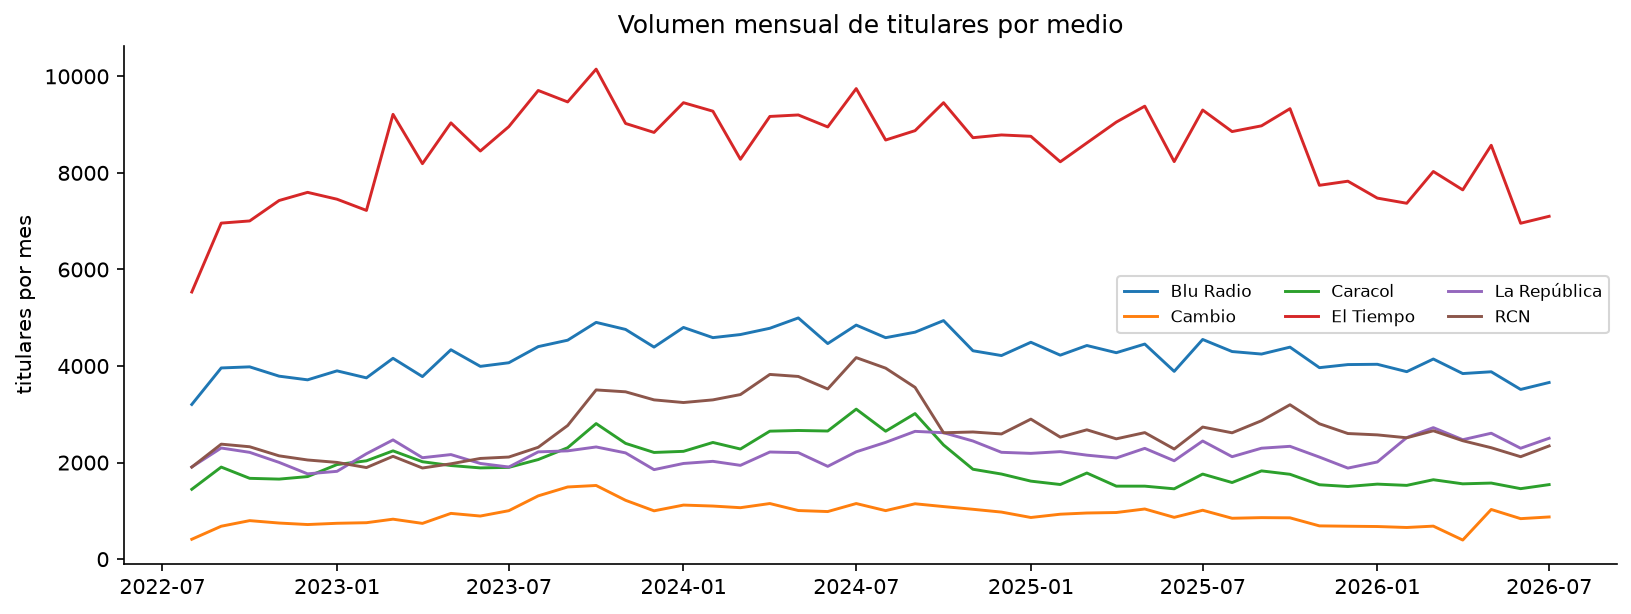
\includegraphics[width=\columnwidth]{figuras/fig01_volumen_mensual.png}
\caption{Volumen mensual de titulares por medio.}
\label{fig:volumen}
\end{figure}

El contenido de servicio representa el 6,9\,\% del corpus, pero se concentra
en pocos medios: en Blu Radio llega al 14,9\,\% (lotería 10,0\,\% y multimedia
4,1\,\%), en El Tiempo al 6,6\,\% (opinión 4,8\,\%) y en Cambio es prácticamente
nulo. Sin esta separación, las frecuencias describirían la oferta de productos
de cada portal y no su manera de informar. Desde aquí, el análisis usa las
916\,452 noticias.

\subsection{Recursos léxicos: tesauros y ontologías}

\subsubsection*{Fundamento}

Un recurso léxico representa conocimiento sobre las palabras y sobre aquello
a lo que se refieren. Interesan aquí tres tipos, de menor a mayor estructura:

\begin{itemize}
\item \textbf{Vocabulario controlado:} lista de términos autorizados para
describir algo, sin relaciones entre ellos.
\item \textbf{Tesauro:} organiza \emph{conceptos}, cada uno con un término
preferente y términos alternativos (sinónimos, variantes), y los relaciona
mediante relaciones jerárquicas (término genérico, BT, y específico, NT) y
asociativas (relacionado, RT). Su referencia normativa es la
ISO~25964~\cite{iso25964}, y en la web se expresa con
SKOS~\cite{skos2009}, que modela los conceptos como
\texttt{skos:Concept} unidos por \texttt{skos:broader} y
\texttt{skos:narrower}, con etiquetas \texttt{skos:prefLabel} y
\texttt{skos:altLabel}.
\item \textbf{Ontología:} según la definición clásica de Gruber, una
«especificación explícita de una conceptualización»~\cite{gruber1993}. Además
de jerarquías, distingue \emph{clases} (tipos de entidad) de \emph{instancias}
(entidades concretas), y puede declarar propiedades y restricciones entre
ellas~\cite{noy2001}.
\end{itemize}

La diferencia práctica es que un tesauro organiza \emph{temas} (de qué trata
un texto), mientras que una ontología organiza \emph{entidades} (quién o qué
aparece en él).

Aplicar estos recursos a un corpus es un \emph{método de diccionario}: un
texto recibe una categoría si contiene alguno de sus términos. Su ventaja es la
transparencia, porque cada asignación se explica por el término que la produjo.
Su riesgo es la validez, ya que un diccionario construido para un dominio puede
fallar en otro; Grimmer y Stewart advierten que estos métodos deben validarse
sobre el corpus concreto antes de interpretar sus resultados~\cite{grimmer2013}.
Por eso todos los recursos se versionan en el repositorio y cada asignación
registra el término y el campo que la originaron.

\subsubsection*{Tesauro temático}

El archivo \texttt{config/topics.yaml} es un tesauro de dos niveles: 7
conceptos generales y 35 específicos, con 209 términos de entrada en total.
En términos de SKOS:

\begin{itemize}
\item Cada tema es un \texttt{skos:Concept} con su nombre como
\texttt{prefLabel}.
\item La relación tema general\,$\to$\,subtema es
\texttt{skos:narrower}. Por ejemplo,
\textit{Seguridad}\,$\to$\,\textit{Conflicto armado}, \textit{Guerrillas},
\textit{Narcotráfico}.
\item Las palabras clave cumplen el papel de \texttt{altLabel}: son los
puntos de entrada léxicos del concepto. Por ejemplo, \textit{Guerrillas} se
activa con \textit{guerrilla}, \textit{eln}, \textit{farc},
\textit{disidencias}.
\end{itemize}

Un titular recibe un subtema cuando alguna de sus palabras clave aparece como
palabra completa (expresión regular con límites de palabra) en el titular, la
ruta de la URL o la sección. El tema general se hereda por la relación
jerárquica, y el etiquetado es multi-etiqueta. Los titulares sin ningún tema no
se descartan: el tesauro cubre política, economía, seguridad, sociedad,
justicia, relaciones internacionales y medio ambiente, y deja fuera por diseño
deportes y entretenimiento.

\subsubsection*{Ontología de actores}

El archivo \texttt{config/actores.yaml} es una ontología ligera con dos niveles
(Tabla~\ref{tab:ontologia}):

\begin{itemize}
\item \textbf{Clases:} 11 tipos de actor.
\item \textbf{Instancias:} 51 actores.
\item \textbf{Relación de pertenencia:} cada actor pertenece a una clase
(equivale a \texttt{rdf:type}).
\item \textbf{Lexicalizaciones:} 204 alias en total. Por ejemplo,
\textit{petro}, \textit{gustavo petro} y \textit{presidente petro} remiten a
la instancia \textit{Gustavo Petro}, de la clase \textit{Gobierno nacional}.
\end{itemize}

\begin{table}[t]
\centering\small
\caption{Clases de la ontología de actores, con el número de instancias y
ejemplos.}
\label{tab:ontologia}
\begin{tabular}{p{2.7cm} r p{3.6cm}}
\toprule
Clase & Inst. & Ejemplos de instancias\\
\midrule
Gobierno nacional       & 6 & Gustavo Petro, Francia Márquez, ministros\\
Oposición política      & 8 & Álvaro Uribe, Centro Democrático\\
Congreso                & 2 & Congreso, partidos tradicionales\\
Rama judicial y Fiscalía & 6 & Fiscalía, Corte Constitucional\\
Órganos de control      & 4 & Procuraduría, Contraloría\\
Fuerza pública          & 2 & Policía, Ejército\\
Grupos armados ilegales & 4 & ELN, disidencias, Clan del Golfo\\
Movimientos sociales    & 6 & indígenas, sindicatos, campesinos\\
Gremios                 & 6 & ANDI, Fenalco, Fedegán\\
Gobiernos locales       & 3 & alcaldes y gobernadores\\
Internacional           & 4 & Estados Unidos, Donald Trump\\
\bottomrule
\end{tabular}
\end{table}

Tres decisiones de diseño responden a la ambigüedad del lenguaje periodístico:

\begin{itemize}
\item \textbf{Precisión antes que cobertura.} Se excluyeron los alias con
lecturas frecuentes ajenas al actor: «fiscal» sin más contexto aparece en
«regla fiscal» y «déficit fiscal», y «galán» tiene usos comunes. Se perdió
cobertura para evitar asignaciones falsas.
\item \textbf{Análisis por clase.} Algunos alias son ambiguos entre instancias:
«uribe» puede referirse a Álvaro o a Miguel Uribe. Ambos pertenecen a la
misma clase, así que el análisis por clase es robusto a esa ambigüedad aunque
la instancia no lo sea.
\item \textbf{Anclaje temporal.} Los cargos corresponden a la ventana del
corpus. Los alias genéricos («fiscal general», «ministro») no dependen de
quién ocupe el cargo.
\end{itemize}

La ontología no se formalizó en OWL porque el análisis solo usa la jerarquía
clase\,$\to$\,instancia y las lexicalizaciones. Su estructura permite, más
adelante, alinear cada instancia con un identificador de Wikidata y heredar
sus propiedades, como el partido o el cargo con sus fechas.

El clasificador de tipos de contenido es, en cambio, un vocabulario controlado
plano: cuatro categorías de servicio con sus términos y rutas de URL, sin
jerarquía.

\subsubsection*{Resultados}

Entre el 27 y el 40\,\% de las noticias contiene al menos un tema del tesauro.
Política es el tema general más frecuente en todos los medios
(Figura~\ref{fig:temas}), y los perfiles difieren de forma marcada:

\begin{itemize}
\item \textbf{La República} es el único medio donde Economía supera el 3\,\%
(8,6\,\%), y casi no cubre seguridad (0,7\,\% frente a 4,8--9,3\,\% en los demás).
\item \textbf{Cambio} tiene la mayor proporción de Política (14,6\,\%) y
Justicia (5,5\,\%).
\end{itemize}

En la ontología, Gustavo Petro es la instancia más mencionada en Blu Radio,
Cambio y Caracol, y Estados Unidos en El Tiempo, La República y RCN. La clase
\textit{Gobierno nacional} aparece en el 10,3\,\% de las noticias de Cambio,
frente a 3,8--6,9\,\% en los demás medios. Estas cifras son descriptivas:
indican qué cubre cada medio, no cómo lo cubre.

\begin{figure}[t]
\centering
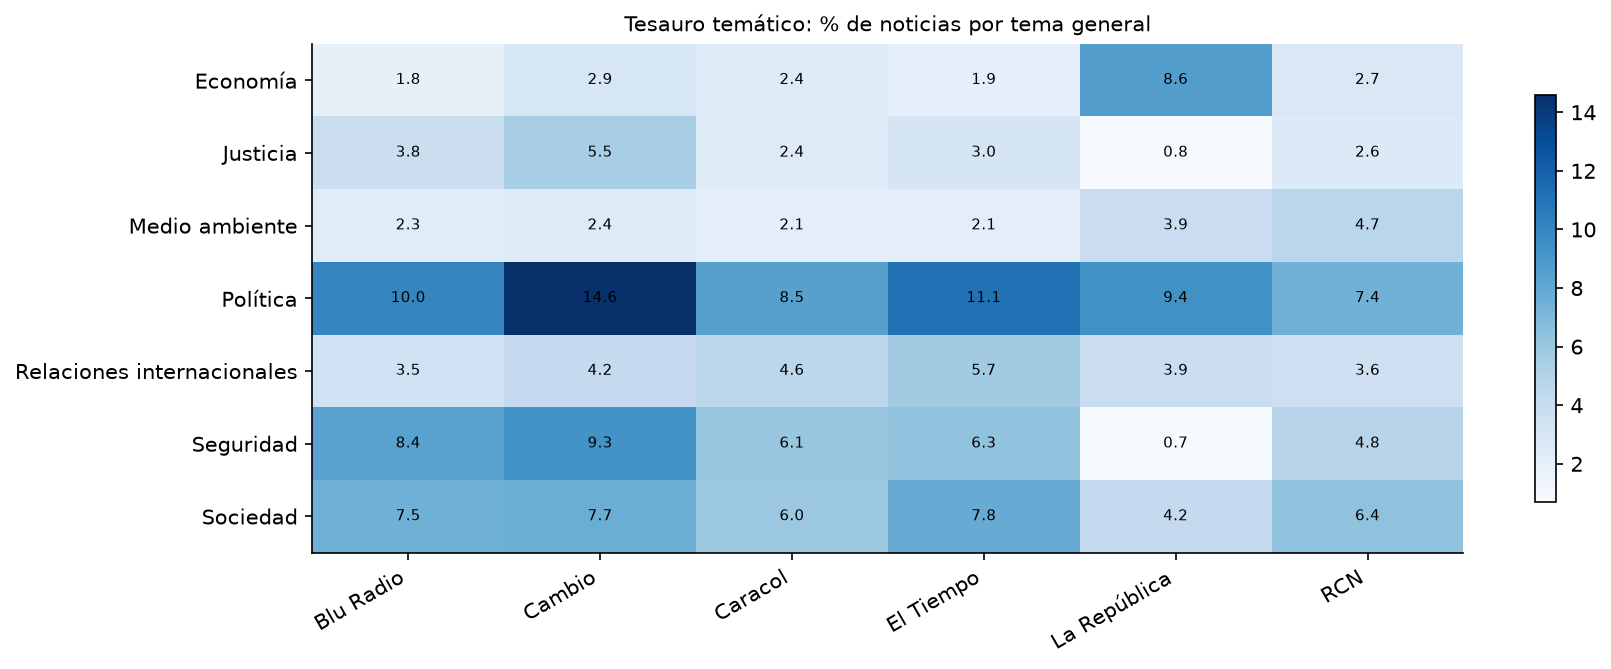
\includegraphics[width=\columnwidth]{figuras/fig03_temas_por_medio.png}
\caption{Porcentaje de noticias por tema general del tesauro.}
\label{fig:temas}
\end{figure}

\subsection{Diversidad léxica}

\textbf{Fundamento.} La diversidad léxica mide qué tan variado es el
vocabulario de un texto: si un medio reutiliza las mismas palabras o recurre a
un repertorio amplio. Sea $N$ el número de tokens de una muestra, $V$ el número
de palabras distintas (tipos) y $V_m$ el número de tipos que aparecen
exactamente $m$ veces. La medida más simple es la razón tipo/token,
$\mathrm{TTR}=V/N$. Su problema es que el vocabulario crece más despacio que
el texto: la ley de Heaps~\cite{heaps1978} establece que $V\approx kN^{\beta}$,
con $0<\beta<1$. Por eso el TTR disminuye con la longitud y dos textos de
distinto tamaño no son comparables~\cite{tweedie1998}. Se usaron cinco medidas
que abordan ese problema de formas distintas:

\begin{itemize}
\item \textbf{Guiraud}~\cite{guiraud1954}: $R=V/\sqrt{N}$, que corrige parcialmente
el efecto del tamaño.
\item \textbf{MATTR}~\cite{covington2010}: el promedio del TTR en ventanas
móviles de $W$ tokens, $\mathrm{MATTR}=\frac{1}{N-W+1}\sum_{i=1}^{N-W+1}
\mathrm{TTR}(t_i,\ldots,t_{i+W-1})$. Como cada ventana tiene el mismo tamaño
($W=500$), la medida no depende de la longitud total.
\item \textbf{MTLD}~\cite{mccarthy2010}: recorre el texto y cuenta cuántos
\emph{factores} se completan, es decir, tramos en los que el TTR acumulado
cae hasta 0,72. $\mathrm{MTLD}=N/F$ es la longitud media de esos tramos: un
valor alto indica que el vocabulario tarda más en repetirse. Se promedia el
recorrido hacia adelante y hacia atrás, y el tramo final se cuenta como
factor parcial.
\item \textbf{$K$ de Yule}~\cite{yule1944}: $K=10^4\,\frac{\sum_m m^2V_m-N}{N^2}$,
que mide la probabilidad de que dos tokens tomados al azar sean la misma
palabra. Un valor \emph{menor} indica \emph{mayor} diversidad, y en teoría no
depende de $N$.
\item \textbf{Proporción de hápax}: $V_1/V$, la fracción de palabras que
aparecen una sola vez.
\end{itemize}

Aun así, para que la comparación sea justa, todas las medidas se calcularon
sobre muestras del mismo tamaño: cinco muestras aleatorias de 200\,000 tokens
por medio, formadas concatenando titulares en orden aleatorio
(Tabla~\ref{tab:div}; las desviaciones entre muestras no superan 0,001 en
MATTR ni 1,8 en MTLD).

\begin{table}[t]
\centering\small
\caption{Diversidad léxica (media de cinco muestras de 200\,000 tokens).
$K$ de Yule: menor es más diverso.}
\label{tab:div}
\begin{tabular}{lrrrr}
\toprule
Medio & TTR & MATTR & MTLD & $K$ Yule\\
\midrule
Cambio       & 0{,}098 & 0{,}629 & 163{,}1 & 119{,}0\\
El Tiempo    & 0{,}102 & 0{,}625 & 158{,}1 & 119{,}8\\
RCN          & 0{,}085 & 0{,}624 & 168{,}3 & 117{,}9\\
La República & 0{,}094 & 0{,}617 & 147{,}3 & 138{,}3\\
Blu Radio    & 0{,}089 & 0{,}585 & 130{,}3 & 117{,}6\\
Caracol      & 0{,}087 & 0{,}576 & 115{,}7 & 129{,}4\\
\bottomrule
\end{tabular}
\end{table}

Se distinguen dos grupos. Cambio, El Tiempo, RCN y La República tienen MATTR
entre 0,617 y 0,629, mientras que Blu Radio y Caracol quedan en 0,576--0,585 y
tienen los MTLD más bajos. Esta menor diversidad persiste aun sin el contenido
de servicio, y coincide con plantillas de titular recurrentes en esos medios
(«pico y placa en\ldots», «quedó en video», «Mañanas Blu»). La República tiene
el $K$ de Yule más alto: concentra su vocabulario en términos económicos
repetidos (dólar, precio, tasas).

\subsection{N-gramas}

\textbf{Fundamento.} Un n-grama es una secuencia de $n$ palabras consecutivas.
Los unigramas describen el vocabulario; los bigramas y trigramas capturan
unidades que no se reducen a sus palabras sueltas: nombres compuestos
(\textit{gustavo petro}), términos (\textit{reforma pensional}) y fórmulas
recurrentes (\textit{pico y placa}). Quitar las \textit{stopwords} antes de
formar n-gramas destruiría expresiones como \textit{reforma a la salud}. Por
eso los n-gramas se forman sobre la secuencia completa y solo se exige que no
empiecen ni terminen en \textit{stopword}: se conserva \textit{reforma a la
salud} y se descarta \textit{de la reforma}. Las frecuencias se reportan por
cada 10\,000 noticias para comparar medios de distinto tamaño.

La Tabla~\ref{tab:ngramas} resume los más frecuentes. Cuatro
patrones se repiten:

\begin{itemize}
\item \textbf{Vocabulario político común:} «gustavo petro», «presidente petro»,
«estados unidos» y «donald trump» están entre los primeros en casi todos los
medios.
\item \textbf{Perfil temático:} La República es económica («petróleo hoy»,
«banco central», «salario mínimo»), RCN es deportiva («selección colombia»,
«luis díaz», «liga betplay») y Cambio es política y judicial («álvaro uribe»,
«corte suprema», «pacto histórico»).
\item \textbf{Autorreferencias} del medio: «mañanas blu», «noticias rcn»,
«emisión noticias».
\item \textbf{Contenido de servicio no cubierto por las reglas:} «pico y placa»
y «precio del dólar» encabezan los trigramas de varios medios. Es un ajuste
pendiente del clasificador.
\end{itemize}

\begin{table*}[t]
\centering\small
\caption{Bigramas más frecuentes por medio (noticias; contenido de servicio excluido).}
\label{tab:ngramas}
\begin{tabular}{llllll}
\toprule
Blu Radio & Cambio & Caracol & El Tiempo & La República & RCN\\
\midrule
mañanas blu        & gustavo petro        & estados unidos   & estados unidos            & estados unidos          & noticias rcn\\
presidente petro   & estados unidos       & presidente petro & gustavo petro             & petróleo hoy            & emisión noticias\\
estados unidos     & álvaro uribe         & gustavo petro    & donald trump              & donald trump            & selección colombia\\
selección colombia & presidente petro     & donald trump     & presidente petro          & américa latina          & luis díaz\\
atlético nacional  & corte suprema        & dólar hoy        & selección colombia        & inteligencia artificial & james rodríguez\\
miguel uribe       & presidente gustavo   & miguel uribe     & presidente gustavo        & gustavo petro           & estados unidos\\
zona rural         & corte constitucional & papa francisco   & luis díaz                 & reino unido             & atlético nacional\\
gustavo petro      & conflicto armado     & redes sociales   & liga betplay              & banco central           & liga betplay\\
\bottomrule
\end{tabular}
\end{table*}

\subsection{Colocaciones}

\textbf{Fundamento.} Una colocación es una combinación de palabras que
aparece junta más de lo que predice el azar. La frecuencia bruta no las
detecta, porque favorece combinaciones de palabras que ya son muy comunes por
separado. La información mutua puntual~\cite{church1990} compara la
probabilidad observada de la pareja con la esperada si las palabras fueran
independientes:
\begin{equation}
\mathrm{PMI}(x,y)=\log_2\frac{P(x,y)}{P(x)\,P(y)}.
\end{equation}
Un PMI de $k$ indica que la pareja aparece $2^k$ veces más de lo esperado. El
PMI sobrevalora los eventos raros (dos palabras que aparecen una sola vez,
juntas, obtienen el máximo), por lo que se exigió una frecuencia mínima de
45 apariciones.

\textbf{Resultados.} Las colocaciones con mayor PMI son nombres propios
(«bankman fried», «btg pactual», «stormy daniels»). Es el comportamiento
esperado: un nombre propio es la colocación más fuerte posible. El resultado es
útil para ampliar la ontología con entidades que todavía no contiene.

\subsection{Coocurrencias}

\textbf{Fundamento.} La hipótesis distribucional sostiene que palabras que
aparecen en contextos parecidos tienen significados
parecidos~\cite{harris1954}, y Firth lo resumió diciendo que una palabra se
conoce por la compañía que mantiene~\cite{firth1957}. Aquí el contexto es el
titular completo. Para un término foco $f$ y otra palabra $w$, se calcula el
PMI a nivel de titular:
\begin{equation}
\mathrm{PMI}(f,w)=\log_2\frac{n_{fw}/n}{(n_f/n)(n_w/n)},
\end{equation}
donde $n$ es el número de titulares y $n_f$, $n_w$ y $n_{fw}$ son los
titulares que contienen $f$, $w$ o ambas. Se usa la presencia y no la
frecuencia, porque una palabra rara vez se repite dentro de un titular. Con un
mínimo de coocurrencias, el resultado describe el campo semántico del término
en el período. La coocurrencia de clases de la ontología en un mismo titular
se reporta además como matriz (pares de tipos de actor).

\textbf{Resultados.} La Tabla~\ref{tab:cooc} muestra los términos con mayor
PMI para seis focos. «Reforma» se asocia con su
trámite legislativo («subcomisión», «ponencia», «hundida») y con sus variantes
(«pensional», «tributaria», «agraria»), y «eln», con los diálogos («garante»,
«negociadores») y con un territorio («arauca»).

\begin{table}[t]
\centering\small
\caption{Términos con mayor PMI de coocurrencia en el mismo titular.}
\label{tab:cooc}
\begin{tabular}{>{\bfseries}l p{5.1cm}}
\toprule
\textnormal{\textbf{Foco}} & \textbf{Coocurrentes}\\
\midrule
petro & alocución, desaprobación, retractarse, alocuciones\\
reforma & subcomisión, pensional, tributaria, hundida, agraria, ponencia\\
eln & garante, cerac, diálogos, negociadores, arauca\\
paz & firmante, comisionado, facilitador, gestores, duradera\\
salud & savia, asmet, mental, reproductiva, magisterio\\
elecciones & atípicas, legislativas, presidenciales, anticipadas\\
\bottomrule
\end{tabular}
\end{table}

% ════════════════════════════════════════════════════════════════════════════
\section{CONJUNTO DE DATOS MEDIDO}

El corpus se entrega preprocesado en la carpeta \texttt{entrega2/} del
repositorio:

\begin{itemize}
\item \texttt{dataset/corpus\_<medio>.parquet}: un archivo por medio, cada uno
por debajo del límite de 100\,MB de GitHub.
\item \texttt{dataset/muestra.csv}: 2\,400 filas legibles en Excel.
\item \texttt{DICCIONARIO\_DATOS.md}: descripción de cada columna.
\item \texttt{metricas/}: las tablas de esta sección.
\end{itemize}

Cada fila es un titular con las siguientes variables:

\begin{itemize}
\item \textbf{Identificación:} \texttt{id}, \texttt{source\_id}, \texttt{medio},
\texttt{government\_id}, \texttt{published\_date}, \texttt{mes}, \texttt{url},
\texttt{section}.
\item \textbf{Texto:} titular original (\texttt{title}), su procedencia
(\texttt{title\_source}), titular normalizado (\texttt{titulo\_limpio}),
\texttt{tokens} y \texttt{tokens\_contenido}.
\item \textbf{Longitudes:} \texttt{n\_caracteres}, \texttt{n\_tokens},
\texttt{n\_tokens\_contenido}.
\item \textbf{Categorías iniciales:} \texttt{tipo\_contenido}, \texttt{temas},
\texttt{temas\_padre}, \texttt{actores}, \texttt{tipos\_actor}.
\end{itemize}

El contenido de servicio se conserva, marcado en \texttt{tipo\_contenido}, para
que cada análisis decida si lo usa. El código que genera el dataset está en el
notebook \path{news-retrieval/notebooks/05-entrega2-eda-representacion.ipynb}
y en el paquete \texttt{news\_corpus.eda}, con 122 pruebas automáticas.

% ════════════════════════════════════════════════════════════════════════════
\section{REPRESENTACIÓN DE LOS TEXTOS}

\subsection{Selección y justificación}

Representar un texto es asignarle un vector numérico sobre el que se pueda
calcular. Cada representación decide qué información conserva. Se compararon
cuatro, ligadas a necesidades distintas del proyecto (Tabla~\ref{tab:rep}):

\begin{itemize}
\item \textbf{BoW} es la línea base interpretable. El sesgo por selección
léxica~\cite{hamborg2019,hamborg2020} se expresa precisamente en qué palabras
se eligen.
\item \textbf{TF-IDF} reduce el peso de lo genérico y destaca lo específico.
\item \textbf{LSA} condensa TF-IDF en dimensiones densas que agrupan palabras
relacionadas.
\item \textbf{FastText}, entrenado sobre el propio corpus, captura similitud
semántica y representa variantes y palabras raras.
\end{itemize}

Quedó implementada como opción una quinta representación contextual,
Sentence-BERT multilingüe~\cite{reimers2019}, prevista para agrupar coberturas
por evento.

\begin{table}[t]
\centering\small
\caption{Representaciones comparadas (916\,452 noticias).}
\label{tab:rep}
\begin{tabular}{lrrl}
\toprule
Técnica & Dim. & Densidad & Interpretable\\
\midrule
BoW              &  44\,204 & 0{,}0168\,\% & sí\\
TF-IDF (1--2 g.) & 197\,921 & 0{,}0052\,\% & sí\\
LSA              &      100 & 100\,\%      & parcial\\
FastText         &      100 & 100\,\%      & por vecinos\\
\bottomrule
\end{tabular}
\end{table}

\subsection{Bolsa de palabras y TF-IDF}

\textbf{Fundamento.} La bolsa de palabras (BoW) representa un titular $d$ como
un vector con una dimensión por palabra del vocabulario; el valor es la
frecuencia $\mathrm{tf}(t,d)$ de la palabra $t$ en el titular. Ignora el orden,
pero conserva qué palabras se eligieron, que es la materia prima del sesgo
léxico. Se incluyeron las palabras que aparecen en al menos cinco titulares.

TF-IDF~\cite{sparckjones1972,salton1988} pondera cada palabra por su
especificidad: una palabra que aparece en todos los titulares
(\textit{colombia}) no distingue a ninguno, y una que aparece en pocos
(\textit{gripen}) caracteriza a los que la contienen. Se usó la variante de
\texttt{scikit-learn} con frecuencia sublineal e IDF suavizado:
\begin{equation}
w_{t,d}=\bigl(1+\ln \mathrm{tf}(t,d)\bigr)\cdot
\Bigl(\ln\tfrac{1+N}{1+\mathrm{df}(t)}+1\Bigr),
\end{equation}
donde $N$ es el número de titulares y $\mathrm{df}(t)$ el número de titulares
que contienen $t$. Cada vector se normaliza a norma euclidiana 1. Se incluyeron
unigramas y bigramas, con $\mathrm{df}\geq5$, y se excluyeron los términos
presentes en más de la mitad de los titulares. Con vectores normalizados, la
similitud entre dos titulares es el coseno del ángulo entre ellos:
\begin{equation}
\cos(\mathbf{a},\mathbf{b})=\frac{\mathbf{a}\cdot\mathbf{b}}
{\lVert\mathbf{a}\rVert\,\lVert\mathbf{b}\rVert},
\end{equation}
que va de 0 (sin palabras en común) a 1 (mismo contenido), porque los pesos
TF-IDF no son negativos.

\textbf{Escasez.} Los titulares son muy cortos (6,5--7,8 palabras de contenido
de media), así que las matrices quedan casi vacías. Un titular activa en
promedio unas siete de las 44\,204 dimensiones de BoW. Dos titulares que tratan
lo mismo con palabras distintas tienen similitud cero. Esta es la razón para
complementar BoW y TF-IDF con representaciones densas.

\subsection{Ejemplo de transformación}

El titular de Cambio «Las razones por las que pidieron a Suecia investigar la
compra de los aviones Gripen por parte de Colombia» se transforma así:

\begin{itemize}
\item \textbf{Tokens de contenido:} \textit{colombia, parte, suecia, razones,
investigar, aviones, compra, pidieron, gripen}.
\item \textbf{BoW:} un 1 en cada una de esas nueve dimensiones.
\item \textbf{TF-IDF:} los pesos mayores son para los bigramas específicos:
\textit{investigar compra} (0,402), \textit{parte colombia} (0,353),
\textit{aviones gripen} (0,314), \textit{compra aviones} (0,313),
\textit{gripen} (0,299).
\item \textbf{FastText:} un vector denso de 100 dimensiones, el promedio de los
vectores de sus palabras menos el vector medio del corpus~\cite{arora2017}, que
comienza en $(0{,}122;\ 0{,}090;\ -0{,}042;\ -0{,}054;\ \ldots)$.
\end{itemize}

\subsection{Recuperación del mismo hecho en distintos medios}

La similitud del coseno entre vectores TF-IDF, restringida a otros medios y a
una ventana de $\pm$2 días, recupera las coberturas de un mismo hecho y
reemplaza el \texttt{evento\_id} manual de la Entrega 1. Para una consulta sobre
la reforma pensional (octubre de 2023), los resultados más similares son de
cuatro medios distintos y cubren el mismo hecho: el aval fiscal del Ministerio
de Hacienda al proyecto (Tabla~\ref{tab:mismo}).

\begin{table}[t]
\centering\small
\caption{Las seis coberturas más similares (TF-IDF) a una consulta sobre la
reforma pensional, en otros medios y $\pm$2 días. Se restituyeron tildes y
puntuación para facilitar la lectura.}
\label{tab:mismo}
\begin{tabular}{l r p{4.1cm}}
\toprule
Medio & Sim. & Titular (reconstruido)\\
\midrule
RCN          & 0{,}43 & Reforma pensional: Ministerio de Hacienda dio el aval fiscal al proyecto en segundo debate\\
Blu Radio    & 0{,}43 & Reforma pensional sería completamente financiable hasta el\ldots: Minhacienda\\
La República & 0{,}38 & El Minhacienda le dio el aval fiscal a la ponencia para segundo debate de la pensional\\
Caracol      & 0{,}26 & Reforma pensional: ¿cuál sería el impacto fiscal de este proyecto?\\
Caracol      & 0{,}25 & Minhacienda da luz verde al proyecto, pero reconoce que nuevo sistema valdrá más\\
Blu Radio    & 0{,}24 & La reforma pensional crea una deuda impagable: Asofondos\\
\bottomrule
\end{tabular}
\end{table}

El ejemplo anticipa el objeto del proyecto. Sobre el mismo hecho, un medio
destaca el aval («dio el aval fiscal»), otro la sostenibilidad («sería
completamente financiable»), otro el costo («valdrá más») y otro la voz crítica
de un gremio («deuda impagable: Asofondos»).

\subsection{Semántica latente (LSA)}

\textbf{Fundamento.} LSA~\cite{deerwester1990} aplica una descomposición en
valores singulares truncada a la matriz TF-IDF $X$:
\begin{equation}
X\approx U_k\Sigma_kV_k^{\top},
\end{equation}
conservando solo las $k=100$ direcciones de mayor varianza. Cada titular pasa
a ser un vector denso de 100 componentes. Las palabras que tienden a aparecer
en los mismos titulares quedan en las mismas componentes, así que dos titulares
pueden parecerse sin compartir palabras. La SVD se ajustó sobre una muestra de
150\,000 noticias.

Para visualizar, se usó t-SNE~\cite{vandermaaten2008}, que proyecta los
vectores a dos dimensiones intentando que los vecinos cercanos sigan siéndolo.
Lo hace minimizando la divergencia de Kullback-Leibler entre las afinidades de
los puntos en el espacio original y en el plano. t-SNE preserva la estructura
\emph{local}, pero no las distancias entre grupos alejados ni su tamaño
relativo, así que solo debe leerse como «qué se agrupa con qué».

\textbf{Resultados.} Las primeras componentes son interpretables:

\begin{itemize}
\item \textbf{2:} Estados Unidos.
\item \textbf{3:} pico y placa.
\item \textbf{4:} el presidente Petro.
\item \textbf{5:} la selección Colombia.
\item \textbf{6:} sucesos (hombre, mujer, accidente).
\item \textbf{7:} dólar y petróleo.
\end{itemize}

La proyección t-SNE~\cite{vandermaaten2008} de 3\,000 noticias
(Figura~\ref{fig:tsne}) muestra que los titulares se agrupan por tema y se
mezclan por medio. La representación captura de qué se habla y no quién lo
publica, que es lo deseable para comparar cómo cuentan los medios un mismo tema.
Hay una excepción visible: un grupo aislado de «medio ambiente» compuesto solo
por titulares de RCN. Coincide con una proporción atípica del subtema «cambio
climático» en ese medio (3,4\,\% de sus noticias), que parece responder a un
formato propio y debe verificarse.

\begin{figure*}[t]
\centering
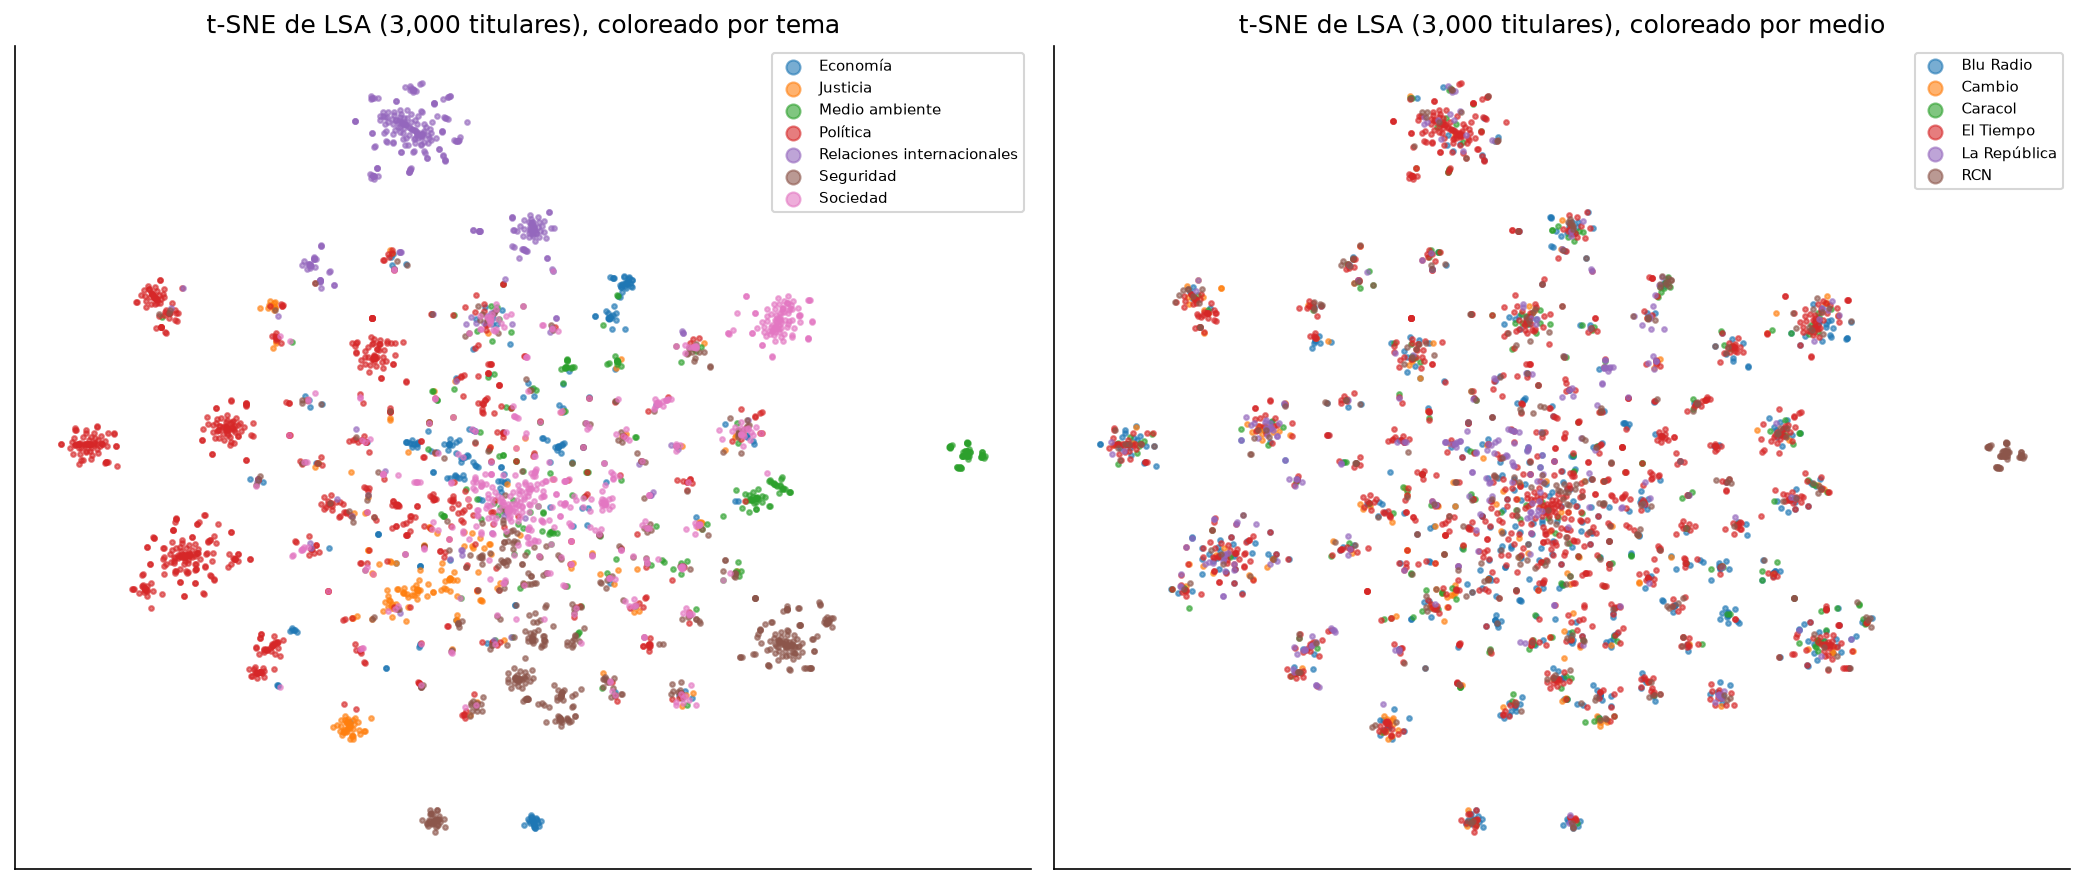
\includegraphics[width=0.92\textwidth]{figuras/fig08_tsne_lsa.png}
\caption{Proyección t-SNE de la representación LSA de 3\,000 noticias,
coloreada por tema (izquierda) y por medio (derecha).}
\label{fig:tsne}
\end{figure*}

\subsection{Embeddings de palabras (FastText)}

\textbf{Fundamento.} Los \emph{embeddings} llevan la hipótesis distribucional a
un vector denso por palabra. El modelo \textit{skip-gram}~\cite{mikolov2013}
aprende los vectores entrenando una tarea auxiliar: predecir las palabras que
rodean a cada palabra dentro de una ventana. Usa muestreo negativo, es decir,
distingue los contextos reales de palabras tomadas al azar. Las palabras que
comparten contextos terminan con vectores cercanos.

FastText~\cite{bojanowski2017} añade información morfológica: el vector de una
palabra es la suma de los vectores de sus n-gramas de caracteres, de 3 a 6.
Por ejemplo, \textit{reforma} incluye \texttt{<re}, \texttt{ref},
\texttt{efo}… Esto permite representar palabras no vistas en el entrenamiento
y comparte información entre variantes (\textit{reforma}, \textit{reformas},
\textit{contrarreforma}), algo útil porque los titulares reconstruidos desde la
URL pierden tildes y pueden truncarse.

Se entrenó sobre las noticias del propio corpus para capturar el vocabulario
colombiano del período, con estos parámetros:

\begin{itemize}
\item 100 dimensiones y ventana de 5.
\item Cinco negativos por ejemplo.
\item Frecuencia mínima de 5.
\item Cinco épocas.
\end{itemize}

Un titular se representa como el promedio de los vectores de sus palabras de
contenido, menos el vector medio del corpus. Esta corrección, una variante
simple de Arora et al.~\cite{arora2017}, elimina la componente común que hace
que todos los promedios se parezcan.

\textbf{Resultados.} Los vecinos más cercanos reflejan relaciones semánticas del
período (Tabla~\ref{tab:ft}). Las subpalabras también introducen vecinos por
forma («salud»\,$\to$\,«talud», «petro»\,$\to$\,«petrovideos»), la contracara de
la misma propiedad que permite manejar variantes.

\begin{table}[t]
\centering\small
\caption{Vecinos más cercanos en FastText (coseno).}
\label{tab:ft}
\begin{tabular}{>{\bfseries}l p{5.2cm}}
\toprule
\textnormal{\textbf{Palabra}} & \textbf{Vecinos}\\
\midrule
eln & disidencias (0,79), farc (0,75), guerrilla (0,74), arauca (0,74)\\
paz & diálogos (0,70), total (0,69), otty (0,68), timochenko (0,65)\\
inflación & desinflación (0,92), estanflación (0,91), deflación (0,86)\\
corrupción & anticorrupción (0,88), corruptos (0,78), escándalo (0,76)\\
salud & secsalud (0,83), minsalud (0,72), eps (0,69)\\
uribe & turbay (0,86), miguel (0,84), álvaro (0,80), uribista (0,68)\\
\bottomrule
\end{tabular}
\end{table}

\subsection{Representaciones contextuales}

\textbf{Fundamento.} En FastText cada palabra tiene un único vector,
independiente de la oración: \textit{paro} recibe el mismo vector en
«paro camionero» y en «paro cardíaco». Los modelos contextuales basados en
\textit{transformers} producen un vector distinto según el contexto.
Sentence-BERT~\cite{reimers2019} ajusta uno de esos modelos con una
arquitectura siamesa para que oraciones con significado parecido queden
cercanas bajo el coseno. Así puede reconocer paráfrasis sin palabras en común
(«Minhacienda da luz verde» y «Hacienda avaló el proyecto»), justo el caso que
TF-IDF no resuelve. Su costo es computacional (un modelo de 470\,MB y
codificación lenta en CPU), por lo que quedó como opción para la fase de
agrupación por eventos.

\subsection{Elección para las siguientes fases}

TF-IDF se mantiene como representación principal para los análisis léxicos y
la recuperación del mismo hecho, por ser interpretable y eficaz con titulares
cortos. FastText aporta la semántica del vocabulario y la robustez frente a
variantes. Las representaciones contextuales se reservan para agrupar
coberturas por evento, donde la paráfrasis entre medios es la norma.

% ════════════════════════════════════════════════════════════════════════════
\section{LIMITACIONES Y PENDIENTES}

\begin{itemize}
\item \textbf{Titulares reconstruidos.} Los titulares vienen de la URL. Algunos
conservan códigos del \textit{slug} (\texttt{rg10}) y otros pueden diferir del
publicado. Su fidelidad debe reportarse con \texttt{validar-titulares}.
\item \textbf{Contenido de servicio.} Formatos como «pico y placa» y «precio del
dólar» aún no se clasifican como servicio.
\item \textbf{Anomalía de RCN.} Hay que verificar a qué se debe la proporción de
«cambio climático» en RCN.
\item \textbf{Recursos léxicos.} El tesauro y la ontología requieren una
validación con una muestra anotada a mano.
\end{itemize}

\bibliographystyle{ieeetr}
\bibliography{referencias}

\end{document}
